\documentclass[12pt]{beamer}
\usepackage[T1]{fontenc} % La police utilisée
\usepackage[utf8]{inputenc} % L'encodage du document
\usepackage[french]{babel} % Des options supplémentaires pour que le document soit en français (noms de sections, etc.)
\usepackage{multirow}

\usepackage{amsmath,amsfonts,amssymb} % Permet l'utilisation de différents symboles mathématiques
\usepackage{hyperref} % Insertion de liens URL
\usepackage{tabularray} % Gestion des tableaux
\usepackage{multirow} % Fusion de lignes dans un tableau
\usepackage{graphicx} % Pour insérer des images
\usepackage{tikz} % Pour faire des graphiques

\title{Document beamer (présentation)}
\author{N. Carré}
\institute{Louis-le-Grand – MPI}
\date{\today}
\titlegraphic{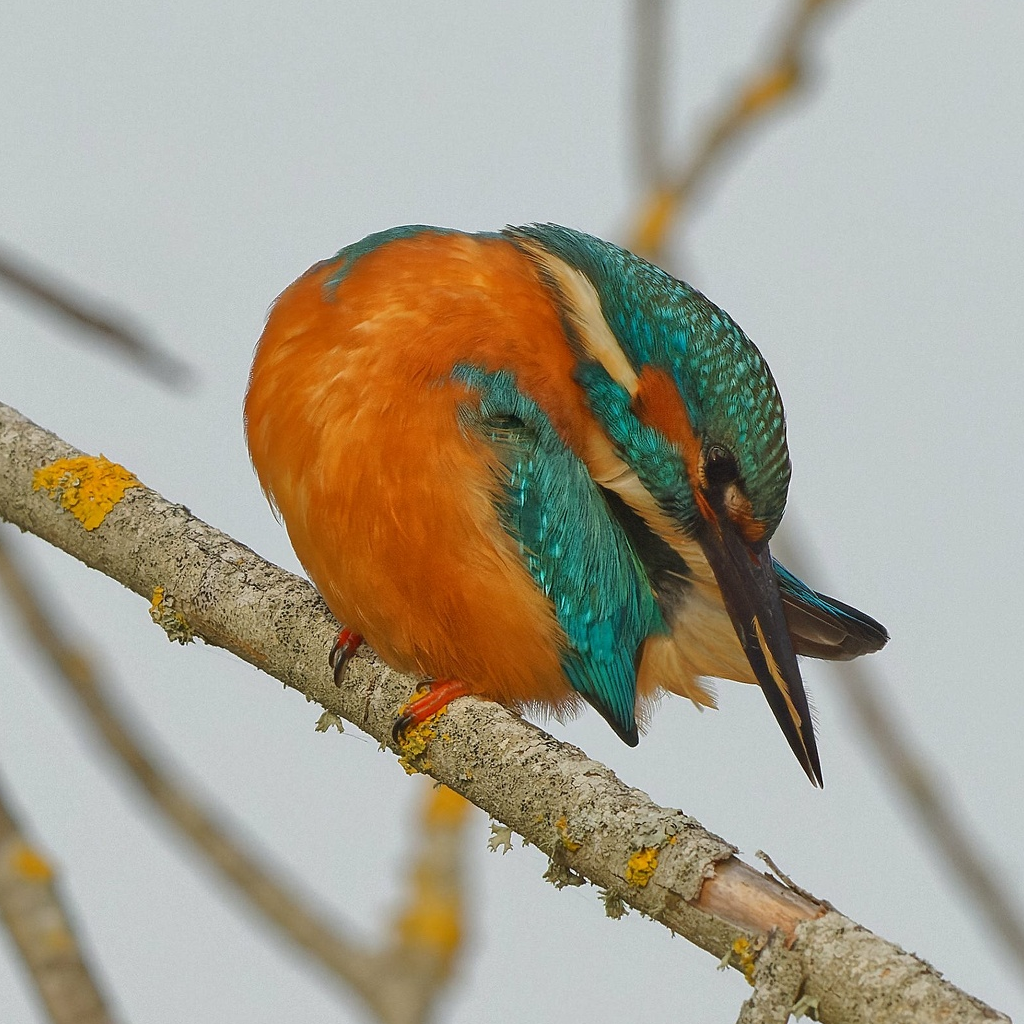
\includegraphics[scale=.1]{martin_pecheur.png}}

%%% Permet de créer des environnements définition/théorème personnalisés %%%
\usepackage[breakable,most]{tcolorbox}

\newtcbtheorem[auto counter, number within = section]{defi}{Définition}{
    % options de style éventuelles
}{def}

\newtcbtheorem[use counter from = defi]{theo}{Théorème}{
    % options de style éventuelles
    colback=red!5!white,
    colframe=black!25,
    coltitle=black
}{theor}
%%%%%%%%%%%%%%%%%%%%%%%%%%%%%%%%%%%%%%%%%%%%%%%%%%%%%%%%%%%%%%%%%%%%%%%%%%%%%%%%%%%

%%% Environnement code %%%
\usepackage{listings}
\usepackage{xcolor}

\lstset{basicstyle=\ttfamily,
	    showstringspaces=false,
        keywordstyle=\color{teal},
        commentstyle=\color{gray},
        stringstyle=\color{violet},
        identifierstyle=\color{blue}}
%%%%%%%%%%%%%%%%%%%%%%%%%%

%%% Environnement pseudo-code %%%
\usepackage[vlined, french, onelanguage]{algorithm2e}
%%%%%%%%%%%%%%%%%%%%%%%%%%%%%%%%%

% Des thèmes graphiques (à essayer)

%\usetheme{default}
%\usetheme{AnnArbor}
%\usetheme{Antibes}
%\usetheme{Bergen}
%\usetheme{Berkeley}
%\usetheme{Berlin}
%\usetheme{Boadilla}
%\usetheme{CambridgeUS}
%%\usetheme{Copenhagen}
%\usetheme{Darmstadt}
%\usetheme{Dresden}
%\usetheme{Frankfurt}
%\usetheme{Goettingen}
%\usetheme{Hannover}
\usetheme{Ilmenau}
%\usetheme{JuanLesPins}
%\usetheme{Luebeck}
%\usetheme{Madrid}
%\usetheme{Malmoe}
%\usetheme{Marburg}
%\usetheme{Montpellier}
%\usetheme{PaloAlto}
%\usetheme{Pittsburgh}
%\usetheme{Rochester}
%\usetheme{Singapore}
%\usetheme{Szeged}
%\usetheme{Warsaw}

% As well as themes, the Beamer class has a number of color themes
% for any slide theme. Uncomment each of these in turn to see how it
% changes the colors of your current slide theme.

%\usecolortheme{albatross}
%\usecolortheme{beaver}
%\usecolortheme{beetle}
%\usecolortheme{crane}
%\usecolortheme{dolphin}
%\usecolortheme{dove}
%\usecolortheme{fly}
%\usecolortheme{lily}
%\usecolortheme{orchid}
%\usecolortheme{rose}
%\usecolortheme{seagull}
%\usecolortheme{seahorse}
%\usecolortheme{whale}
%\usecolortheme{wolverine}



\begin{document}
\setbeamertemplate{navigation symbols}{\Large\insertframenumber/\inserttotalframenumber} % Affiche des numéros de page
\setbeamertemplate{headline}{} % Commenter pour ajouter une entête contenant le plan
\setbeamertemplate{footline}{} % Commenter pour ajouter un pied de page contenant le titre et l'auteur
%\setbeamertemplate{footline}[page number]

\frame{\titlepage} % Affiche la diapo de titre

\begin{frame}
\tableofcontents % Table des matières : il faut compiler deux fois pour la prendre en compte
\end{frame}

\AtBeginSection[] % Permet de rajouter une diapo de plan à chaque début de section (facultatif)
{
 \begin{frame}<beamer>
 \tableofcontents[currentsection]
 \end{frame}
}
\section{Introduction}
\subsection{Schéma d'une diapo}
\begin{frame}
\frametitle{Un titre}
Un contenu

\begin{itemize}
\item des items
\item d'autres items
\end{itemize}
\end{frame}

\subsection{Pause}

\begin{frame}
\frametitle{Temporiser le contenu}
Ce texte est sur la première diapo.\pause
\begin{itemize}
\item ce texte est sur la suivante \pause
\item ce texte arrive ensuite \pause
\item vous avez compris l'idée
\end{itemize}
\end{frame}

\begin{frame}
\frametitle{On peut ne mettre certains objets que sur certaines diapos}
\texttt{\textbackslash only} marche à l'intérieur d'autres environnements  (par exemple \texttt{tikzpicture}).
\begin{itemize}
\item \only<1>{cet item va disparaître}
\item \only<2-3>{cet item restera}
\item \only<3>{dernier item}
\end{itemize}

\end{frame}

\begin{frame}
\frametitle{ou cacher/faire apparaître}
\texttt{\textbackslash uncover} permet de faire ces modifications
\begin{itemize}
\item \uncover<1-2>{premier item}
\item \uncover<2->{deuxième item}
\item \uncover<3>{troisième item}
\end{itemize}

Ici, la différence avec \texttt{only} est que les objets sont présents mais invisibles.
\end{frame}


\section{Quelques environnements supplémentaires}

\subsection{Définition}
\begin{frame}
\frametitle{Une définition}
On a les définitions suivantes :
\begin{defi}{}{}
Une définition numérotée
\end{defi}

\begin{defi*}{}
Une définition non numérotée
\end{defi*}
\end{frame}

\subsection{Théorème}

\begin{frame}
\frametitle{Un théorème}

\begin{theo}{}{}
Un théorème numéroté
\end{theo}
\end{frame}

\subsection{Du code}

\begin{frame}[fragile]
\frametitle{Du code}

Attention, l'option \verb"[fragile]" est nécessaire.

\begin{lstlisting}[language=c, frame=single, numbers=left]
int main(void){
    int x = 5; // Je pose x qui vaut 5.
    printf("La valeur de x est %d\n", x);
    return EXIT_SUCCESS;
}
\end{lstlisting}
\end{frame}

\subsection{Du pseudo-code}

\begin{frame}
\frametitle{Pseudo-code}

\begin{algorithm}[H]
  \KwData{Ce document}
  \KwResult{Comment écrire un algorithme}
  On crée l'environnement\\
  \While{on n'est pas à la fin}{
    On lit une phrase\\
    \eIf{on a compris}{
      $x \leftarrow x + 1$\\
      On passe à la section suivante.
    }{
      \If{on est perdu}{
      	On recommence depuis le début.
      }
    }
  }
  \caption{Comment écrire un algorithme}
\end{algorithm}
\end{frame}

\begin{frame}
\frametitle{Numéroter les lignes}
\LinesNumbered
\begin{algorithm}[H]
  \KwData{Ce document}
  \KwResult{Comment écrire un algorithme}
  On crée l'environnement\\
  \While{on n'est pas à la fin}{
    On lit une phrase\\
    \eIf{on a compris}{
      $x \leftarrow x + 1$\\
      On passe à la section suivante.
    }{
      \If{on est perdu}{
      	On recommence depuis le début.
      }
    }
  }
  \caption{Comment écrire un algorithme}
\end{algorithm}
\end{frame}

\end{document}
